\chapter{Indledning}

Med udgangspunkt i børnesikkerhed i hjemmet vil vi udvikle et produkt, som kan hjælpe familier med børn, til at få et mere sikkert hjem.

Konkret konstrueres følgende:

\begin{itemize}
\item Afbryder til valgt 230V stikkontakt
\subitem Beskyttelse mod kogeplader og lignende
\item Låsemekanisme til at låse skabe og skuffer
\subitem Aflåsning af skuffe med køkkenknive
\item Sensor system til at detektere brand $CO_2$, temperature, bevægelse og lyd
\subitem Beskyttelse mod brand, indbrud og en udvidet babymonitor
\end{itemize}

Systemet skal være nemt at sætte op og skal kommunikere over det eksisterende 230V vekselspændings netværk i hus installationen.

En central enhed håndterer styringen i mellem enhederne og der skal være mulighed for at tilkoble en computer som kan bruges til at styre og aflæse systemet. Hele systemet aktiveres med et kodetryk.
\\
\\
\begin{figure}[h] \centering
\fbox{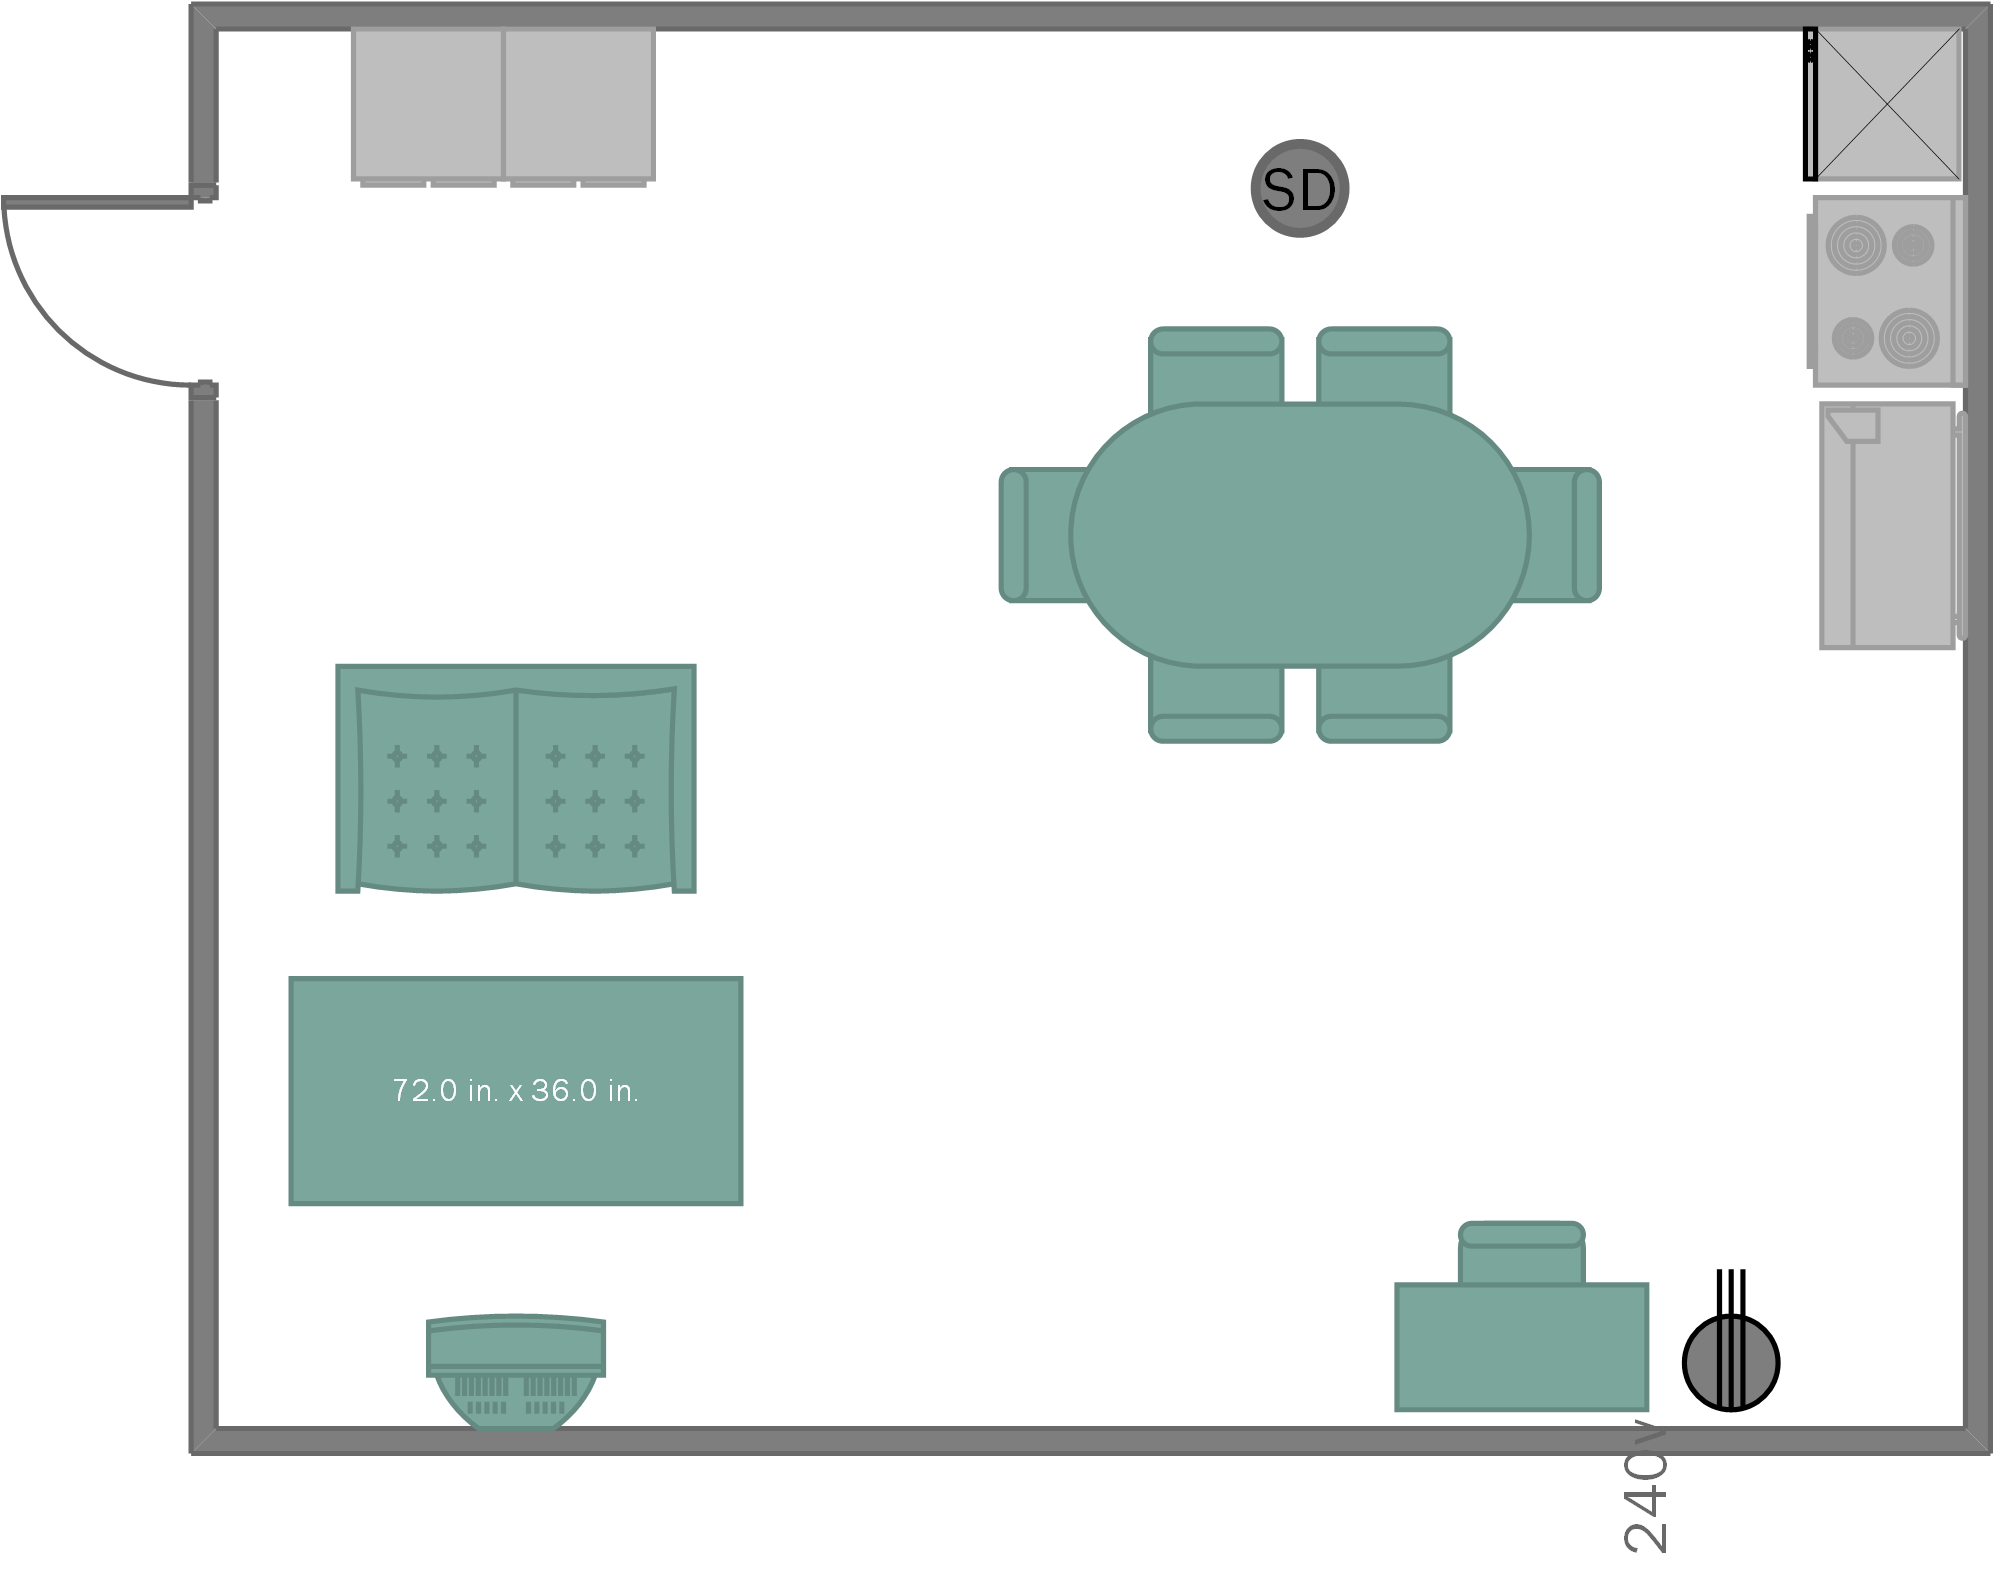
\includegraphics[width=0.6\textwidth]{billeder/Plan_tegning}}
\caption{Plan tegning}
\label{lab:plantegning}
\end{figure}
